%% LaTeX2e class for student theses
%% methodology.tex
%%
%% Berlin University of Applied Sciences and Technology
%% Fachbereich 6: Informatik und Medien
%% Cognitive Algorithms Lab (Calgo Lab)
%%
%% Prof. Dr. Felix Bießmann
%% felix.biessmann@bht-berlin.de
%%
%% Version 0.1, 2023-03-26
%%
%% -----------------------------------------------------


\chapter{Methodology}
\label{ch:methodology}

Lorem Ipsum


\section{Hypothesis}
\label{sec:methodology:hypothesis}

Lorem Ipsum


\section{Some Examples}
\label{sec:methodology:important_stuff}

Lorem Ipsum


\subsection{Abbreviations}
\label{sec:methodology:example:abbreviation}
%
Abbreviations can be useful and are automatically handled, see: \gls{ML}, \gls{ML}.

One can also define plurals: \glspl{CNN}, \gls{CNN}, \glspl{CNN}.


\subsection{Figure}
\label{sec:methodology:example:figure}
%
Figure \ref{fig:cnn} visualizes how \glspl{CNN} work.

\begin{figure}[h]%
	\centering
	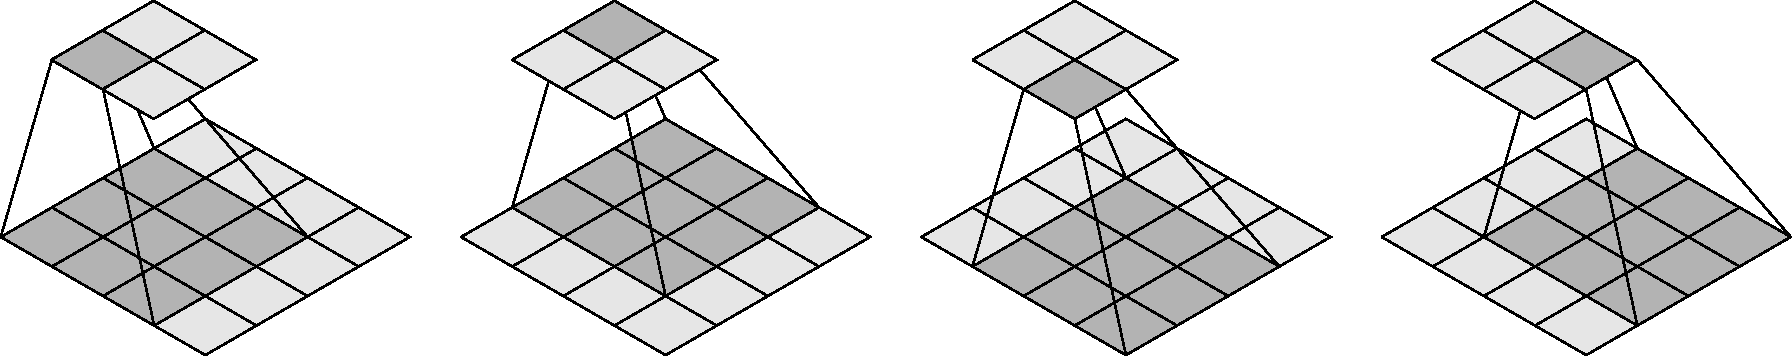
\includegraphics[width=\textwidth]{figures/cnn}
	\caption{
		CNN. Some more description.
	}
	\label{fig:cnn}
\end{figure}
%


\subsection{Table}
\label{sec:methodology:example:table}
%
Table \ref{tab:example-table} has two columns and three rows.

\begin{table}[h]
	\centering
	\begin{tabular}{rl}
		\toprule
		Column 1 & Column 2 \\
		\midrule
		1        & A        \\
		2        & B        \\
		3        & C        \\
		\bottomrule
	\end{tabular}
	\caption{Table. Detailed description.}
	\label{tab:example-table}
\end{table}


\subsection{Math}
\label{sec:methodology:example:math}
%
Equations \ref{eq:precision} and \ref{eq:recall} are important.
%
\begin{equation}
	precision = \frac{TP}{TP + FP}
	\label{eq:precision}
\end{equation}
%
\begin{equation}
	recall = \frac{TP}{TP + FN}
	\label{eq:recall}
\end{equation}
%


\subsection{Citation}
\label{sec:methodology:example:citation}
%
Some references about data imputation~\cite{jagerBenchmarkDataImputation2021}, the GreenDB~\cite{jagerGreenDBDatasetBenchmark2022, jagerGreenDBProductbyProductSustainability2022, gossenNudgingSustainableConsumption2022}, or how to scale \glspl{NN}~\cite{jagerParallelizedTrainingDeep2018}.


\subsection{Footnote}
\label{sec:methodology:example:footnote}
%
Footnotes can be used to add additional information\footnote{Additional information about XYZ.} or links\footnote{\url{calgo-lab.de}}.


\section{Summary}
\label{sec:methodology:summary}

It can be helpful to summarize what is written here.